\RequirePackage{plautopatch}
\documentclass[platex,dvipdfmx,a4paper]{jsarticle}

\usepackage{amsmath}
\usepackage{amsfonts}
\usepackage{amssymb}
\usepackage[dvipdfmx]{graphicx}

\newcommand{\hb}[2]{\frac{\sectionial #1}{\sectionial #2}}
\newcommand{\bbn}[2]{\frac{d #1}{d #2}}
\newcommand{\hhb}[2]{\frac{\sectionial^2 #1}{\sectionial #2^2}}
\newcommand{\bbbn}[2]{\frac{d^2 #1}{d #2^2}}
\newcommand{\vectxy}[2]{\begin{pmatrix}#1\\#2\end{pmatrix}}
\newcommand{\vectxyz}[3]{\begin{pmatrix}#1\\#2\\#3\end{pmatrix}}
\newcommand{\vect}[1]{\boldsymbol{\mathrm{#1}}}

\newcommand{\ssum}[3]{\sum_{#1=#2}^#3}

\title{物理数学II演習レポート3}
\author{嶋田 悠音}
\date{2026年6月26日}

  

\begin{document}
  \maketitle
  \subsection*{問題2}
  \begin{figure}[h]
    \centering
    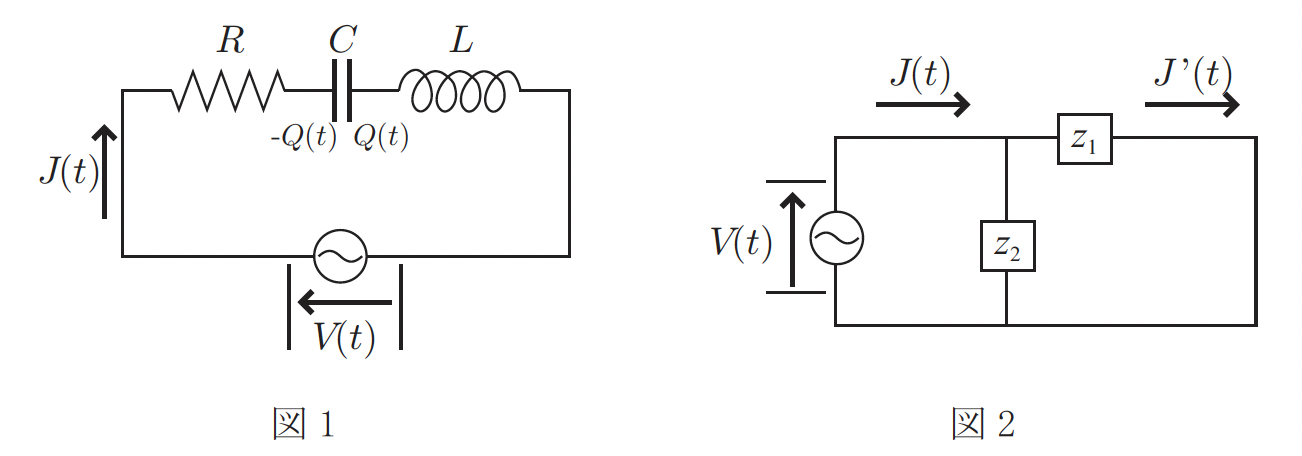
\includegraphics[width=15cm]{math2_3.png}
  \end{figure}
  \subsubsection*{I(a)}
  抵抗、コンデンサー、コイルを直列に繋いだ図1のような回路を考える。\\
  コンデンサーに溜まった電荷を$Q(t)$として、$J(t),Q(t)$の関係は次のようになる：
  \begin{align*}
    J(t)=-\bbn{Q(t)}{t}。
  \end{align*}
  各素子にかかる電圧を、電流の向きに沿った電圧降下として書く。抵抗、コイルについてはそれぞれ
  \begin{align*}
    V_R(t)=RJ(t),\quad V_L(t)=L\bbn{J(t)}{t}
  \end{align*}
  である。また、コンデンサーでは左側極板が$-Q(t)$、右側極板が$Q(t)$であるから、電流の向きに沿った電圧降下は
  \begin{align*}
    V_C(t)=-\frac{Q(t)}{C}
  \end{align*}
  である。したがって、Kirchhoffの電圧則より、入力電圧$V(t)$は
  \begin{align*}
    V(t)=RJ(t)-\frac{Q(t)}{C}+L\bbn{J(t)}{t}
  \end{align*}
  と書ける。以上より、求める関係式は以下：
  \begin{align*}
    J(t)=-\bbn{Q(t)}{t},\qquad
    V(t)=RJ(t)-\frac{Q(t)}{C}+L\bbn{J(t)}{t}。
  \end{align*}

  \subsubsection*{I(b)}

  入力電圧が
  \begin{align*}
    V(t)=\upsilon e^{\mathrm{i}\omega t}
  \end{align*}
  で与えられたとき、電流が
  \begin{align*}
    J(t)=je^{\mathrm{i}\omega t}
  \end{align*}
  の形で応答するとして、複素インピーダンス$z=\upsilon/j$を求める。

  まず、I(a)で得た
  \begin{align*}
    J(t)=-\bbn{Q(t)}{t}
  \end{align*}
  より、
  \begin{align*}
    je^{\mathrm{i}\omega t}=-\bbn{Q(t)}{t}
  \end{align*}
  である。したがって、同じ角振動数の定常応答について
  \begin{align*}
    Q(t)=-\frac{j}{\mathrm{i}\omega}e^{\mathrm{i}\omega t}
  \end{align*}
  と書ける。これをI(a)で得た回路方程式に代入する：
  \begin{align*}
    \upsilon e^{\mathrm{i}\omega t}
    &= Rje^{\mathrm{i}\omega t}
      -\frac{1}{C}\left(-\frac{j}{\mathrm{i}\omega}e^{\mathrm{i}\omega t}\right)
      +L\bbn{}{t}\left(je^{\mathrm{i}\omega t}\right) \\
    &= \left(R+\frac{1}{\mathrm{i}\omega C}+\mathrm{i}\omega L\right)je^{\mathrm{i}\omega t}。
  \end{align*}
  両辺を$je^{\mathrm{i}\omega t}$で割ると、複素インピーダンスは
  \begin{align*}
    z(\omega)
    &=\frac{\upsilon}{j} \\
    &=R+\mathrm{i}\omega L+\frac{1}{\mathrm{i}\omega C} \\
    &=R+\mathrm{i}\left(\omega L-\frac{1}{\omega C}\right)
  \end{align*}
  である。

  \subsubsection*{I(c)}

  入力電圧$V(t)$のFourier変換が$\upsilon(\omega)$で与えられているとき、出力電流$J(t)$を積分表示で表す。Fourier逆変換を
  \begin{align*}
    V(t)=\frac{1}{2\pi}\int_{-\infty}^{\infty}\upsilon(\omega)e^{\mathrm{i}\omega t}\,d\omega
  \end{align*}
  と書く。回路は線形であるから、各角振動数成分は独立に応答する。角振動数$\omega$の成分については、I(b)より
  \begin{align*}
    j(\omega)=\frac{\upsilon(\omega)}{z(\omega)}
  \end{align*}
  である。したがって、出力電流は
  \begin{align*}
    J(t)
    =\frac{1}{2\pi}\int_{-\infty}^{\infty}
    \frac{\upsilon(\omega)}{R+\mathrm{i}\omega L+\frac{1}{\mathrm{i}\omega C}}
    e^{\mathrm{i}\omega t}\,d\omega
  \end{align*}
  と表される。

  \subsubsection*{II(d)}
  複素インピーダンス$z_1,z_2$を持つ素子を並列につなげて図2のような回路を作る。\\
  抵抗、コンデンサー、コイルそれぞれの複素インピーダンスを求める。入力電圧と電流が次のようになるとする：
  \begin{align*}
    V(t)=\upsilon e^{\mathrm{i}\omega t},\quad
    J(t)=je^{\mathrm{i}\omega t}。
  \end{align*}

  抵抗ではOhmの法則$V(t)=RJ(t)$が成り立つので、
  \begin{align*}
    z_R(\omega)=R
  \end{align*}
  である。コンデンサーでは、電圧と電荷の関係を$V(t)=Q(t)/C$とすれば、
  \begin{align*}
    J(t)=\bbn{Q(t)}{t}=C\bbn{V(t)}{t}
  \end{align*}
  である。したがって、
  \begin{align*}
    J(t)
    &=C\bbn{}{t}\left(\upsilon e^{\mathrm{i}\omega t}\right) \\
    &=\mathrm{i}\omega C\upsilon e^{\mathrm{i}\omega t}
  \end{align*}
  となるので、
  \begin{align*}
    j=\mathrm{i}\omega C\upsilon
  \end{align*}
  である。よって、コンデンサーの複素インピーダンスは
  \begin{align*}
    z_C(\omega)=\frac{\upsilon}{j}=\frac{1}{\mathrm{i}\omega C}
  \end{align*}
  である。コイルでは$V(t)=L\bbn{J(t)}{t}$であるから、
  \begin{align*}
    V(t)
    &=L\bbn{}{t}\left(je^{\mathrm{i}\omega t}\right) \\
    &=\mathrm{i}\omega Lje^{\mathrm{i}\omega t}
  \end{align*}
  となる。したがって、コイルの複素インピーダンスは
  \begin{align*}
    z_L(\omega)=\mathrm{i}\omega L
  \end{align*}
  である。

  \subsubsection*{II(e)}
  両素子は並列であるから、各素子にかかる電圧は同じであり、これを$V(t)$とする。角振動数$\omega$の定常応答を考えると、各枝の電流は
  \begin{align*}
    j_1=\frac{\upsilon}{z_1},\qquad
    j_2=\frac{\upsilon}{z_2}
  \end{align*}
  である。全電流$j$は枝電流の和なので、
  \begin{align*}
    j
    &=j_1+j_2 \\
    &=\frac{\upsilon}{z_1}+\frac{\upsilon}{z_2} \\
    &=\upsilon\left(\frac{1}{z_1}+\frac{1}{z_2}\right)。
  \end{align*}
  また、出力電流を$z_1$側の電流とすれば、
  \begin{align*}
    j'=j_1=\frac{\upsilon}{z_1}
  \end{align*}
  である。したがって、入出力比は
  \begin{align*}
    \frac{j'}{j}
    &=\frac{\frac{\upsilon}{z_1}}{\upsilon\left(\frac{1}{z_1}+\frac{1}{z_2}\right)} \\
    &=\frac{\frac{1}{z_1}}{\frac{z_1+z_2}{z_1z_2}} \\
    &=\frac{z_2}{z_1+z_2}
  \end{align*}
  である。

  \subsubsection*{II(f)}

  $z_1,z_2$をコンデンサーとコイルにした場合の入出力比$j'/j$の角振動数依存性を調べる。II(e)より、$J'(t)$を$z_1$側の電流と読むと、
  \begin{align*}
    \frac{j'}{j}=\frac{z_2}{z_1+z_2}
  \end{align*}
  である。

  まず、$z_1$をコンデンサー、$z_2$をコイルとする。このとき、
  \begin{align*}
    z_1=\frac{1}{\mathrm{i}\omega C},\qquad
    z_2=\mathrm{i}\omega L
  \end{align*}
  である。したがって、
  \begin{align*}
    \frac{j'}{j}
    &=\frac{\mathrm{i}\omega L}{\frac{1}{\mathrm{i}\omega C}+\mathrm{i}\omega L} \\
    &=\frac{\omega L}{\omega L-\frac{1}{\omega C}} \\
    &=\frac{\omega^2LC}{\omega^2LC-1}。
  \end{align*}
  ここで、共鳴角振動数$\omega_0$を
  \begin{align*}
    \omega_0=\frac{1}{\sqrt{LC}}
  \end{align*}
  により定めると、
  \begin{align*}
    \frac{j'}{j}
    =\frac{\left(\frac{\omega}{\omega_0}\right)^2}{\left(\frac{\omega}{\omega_0}\right)^2-1}
  \end{align*}
  と書ける。低周波極限では
  \begin{align*}
    \lim_{\omega\to0}\frac{j'}{j}=0
  \end{align*}
  であり、高周波極限では
  \begin{align*}
    \lim_{\omega\to\infty}\frac{j'}{j}=1
  \end{align*}
  である。したがって、この場合は低周波成分を抑え、高周波成分を通す性質を持つ。ただし、理想的な抵抗なしのLC回路では、$\omega=\omega_0$で共鳴により振幅が発散する。

  次に、$z_1$をコイル、$z_2$をコンデンサーとする。このとき、
  \begin{align*}
    z_1=\mathrm{i}\omega L,\qquad
    z_2=\frac{1}{\mathrm{i}\omega C}
  \end{align*}
  である。したがって、
  \begin{align*}
    \frac{j'}{j}
    &=\frac{\frac{1}{\mathrm{i}\omega C}}{\mathrm{i}\omega L+\frac{1}{\mathrm{i}\omega C}} \\
    &=\frac{1}{1-\omega^2LC} \\
    &=\frac{1}{1-\left(\frac{\omega}{\omega_0}\right)^2}。
  \end{align*}
  低周波極限では
  \begin{align*}
    \lim_{\omega\to0}\frac{j'}{j}=1
  \end{align*}
  であり、高周波極限では
  \begin{align*}
    \lim_{\omega\to\infty}\frac{j'}{j}=0
  \end{align*}
  である。したがって、この場合は低周波成分を通し、高周波成分を抑える性質を持つ。こちらの場合も、理想的な抵抗なしのLC回路では、$\omega=\omega_0$で共鳴により振幅が発散する。

  以上より、$z_1$をコンデンサー、$z_2$をコイルとした場合は高周波側を通すフィルタとして働き、$z_1$をコイル、$z_2$をコンデンサーとした場合は低周波側を通すフィルタとして働くことがわかる。
\end{document}
